%%%%%%%%%%%%%%%%%%%%%%%%%%%%%%%%%%%%%%%%%
% Jacobs Landscape Poster
% LaTeX Template
% Version 1.1 (14/06/14)
%
% Created by:
% Computational Physics and Biophysics Group, Jacobs University
% https://teamwork.jacobs-university.de:8443/confluence/display/CoPandBiG/LaTeX+Poster
%
% Further modified by:
% Nathaniel Johnston (nathaniel@njohnston.ca)
%
% This template has been downloaded from:
% http://www.LaTeXTemplates.com
%
% License:
% CC BY-NC-SA 3.0 (http://creativecommons.org/licenses/by-nc-sa/3.0/)
%
%%%%%%%%%%%%%%%%%%%%%%%%%%%%%%%%%%%%%%%%%

%----------------------------------------------------------------------------------------
%	PACKAGES AND OTHER DOCUMENT CONFIGURATIONS
%----------------------------------------------------------------------------------------

\documentclass[final]{beamer}

\usepackage[scale=1.24]{beamerposter} % Use the beamerposter package for laying out the poster
\usepackage{amsmath}
\usepackage{epsfig}


\usetheme{confposter} % Use the confposter theme supplied with this template

\setbeamercolor{block title}{fg=ngreen,bg=white} % Colors of the block titles
\setbeamercolor{block body}{fg=black,bg=white} % Colors of the body of blocks
\setbeamercolor{block alerted title}{fg=white,bg=dblue!70} % Colors of the highlighted block titles
\setbeamercolor{block alerted body}{fg=black,bg=dblue!10} % Colors of the body of highlighted blocks
% Many more colors are available for use in beamerthemeconfposter.sty

%-----------------------------------------------------------
% Define the column widths and overall poster size
% To set effective sepwid, onecolwid and twocolwid values, first choose how many columns you want and how much separation you want between columns
% In this template, the separation width chosen is 0.024 of the paper width and a 4-column layout
% onecolwid should therefore be (1-(# of columns+1)*sepwid)/# of columns e.g. (1-(4+1)*0.024)/4 = 0.22
% Set twocolwid to be (2*onecolwid)+sepwid = 0.464
% Set threecolwid to be (3*onecolwid)+2*sepwid = 0.708

\newlength{\sepwid}
\newlength{\onecolwid}
\newlength{\twocolwid}
\newlength{\threecolwid}
\setlength{\paperwidth}{48in} % A0 width: 46.8in
\setlength{\paperheight}{36in} % A0 height: 33.1in
\setlength{\sepwid}{0.024\paperwidth} % Separation width (white space) between columns
\setlength{\onecolwid}{0.22\paperwidth} % Width of one column
\setlength{\twocolwid}{0.464\paperwidth} % Width of two columns
\setlength{\threecolwid}{0.708\paperwidth} % Width of three columns
\setlength{\topmargin}{-0.5in} % Reduce the top margin size
%-----------------------------------------------------------

\usepackage{graphicx}  % Required for including images

\usepackage{booktabs} % Top and bottom rules for tables

%----------------------------------------------------------------------------------------
%	TITLE SECTION
%----------------------------------------------------------------------------------------

\title{Watching Videos with Certain and Constant Quality: PID-based Quality Control Method} % Poster title

\author{Yuhang Song$^*$, Mai Xu$^{*~\dag}$, and Shengxi Li$^*$} % Author(s)

\institute{$^*$ School of Electronic and Information Engineering, Beihang University \\
$\dag$ EDA Lab, Research Institute of Tsinghua University in Shenzhen} % Institution(s)

%----------------------------------------------------------------------------------------

\begin{document}

\addtobeamertemplate{block end}{}{\vspace*{2ex}} % White space under blocks
\addtobeamertemplate{block alerted end}{}{\vspace*{2ex}} % White space under highlighted (alert) blocks
\newcommand{\argmin}{\operatornamewithlimits{argmin}}

\setlength{\belowcaptionskip}{2ex} % White space under figures
\setlength\belowdisplayshortskip{2ex} % White space under equations

\begin{frame}[t] % The whole poster is enclosed in one beamer frame

\begin{columns}[t] % The whole poster consists of three major columns, the second of which is split into two columns twice - the [t] option aligns each column's content to the top

\begin{column}{\sepwid}\end{column} % Empty spacer column

\begin{column}{\onecolwid} % The first column

%----------------------------------------------------------------------------------------
%	OBJECTIVES
%----------------------------------------------------------------------------------------

\begin{alertblock}{Objectives}

In video coding, compressed videos with certain and constant quality can ensure quality of experience (QoE). To this end, we propose in this paper a novel PID-based quality control (PQC) method for video coding. Specifically, a formulation is modelled to control quality of video coding with two objectives: minimizing control error and quality fluctuation. Then, we apply the Laplace domain analysis to model the relationship between quantization parameter (QP) and control error in this formulation. Given the relationship between QP and control error, we propose a solution to the PQC formulation, such that videos can be compressed at certain and constant quality. Finally, experimental results show that our PQC method is effective in both control accuracy and quality fluctuation.

\end{alertblock}

%----------------------------------------------------------------------------------------
%	INTRODUCTION
%----------------------------------------------------------------------------------------

\begin{block}{Formulation of quality control}

In video coding, there are two main objectives for quality control:

$\textbf{Objective I}$: Minimizing the error between the actual and target quality, averaged over all frames.

$\textbf{Objective II}$: Minimizing the fluctuation of quality along with frames.

The above two objectives can be achieved by predicting the optimal $\mathrm{QP}$ before encoding each frame. In other words, before encoding the $t$-th frame, we need to estimate the best $\mathrm{QP}$ value for this frame, which is denoted by $\mathrm{QP}_{t}$. Assuming that $T$ is the target distortion and $D_t$ is the distortion of the $t$-th frame, the quality control can be formulated by
\begin{equation}
\label{quality-control-formulation}
\footnotesize{
\mathrm{QP}_{t}=\argmin_{\mathrm{QP}} \lbrace \underbrace{\lambda \cdot \underbrace{(D_{t}(\mathrm{QP})-T)}_{\textbf{Objective I}}+(1-\lambda) \cdot \underbrace{\dfrac{dD_{t}(\mathrm{QP})}{dt}}_{\textbf{Objective II}}}_{e_t} \rbrace,
}
\end{equation}
where $(D_{t}(\mathrm{QP})-T)$ modells the error between the actual and target quality ($\textbf{Objective I}$), while $\frac{dD_{t}(\mathrm{QP})}{d_t}$ modells the fluctuation of quality ($\textbf{Objective II}$). In addition, $\lambda$ represents the trade-off between the two objectives, and $e_t$ denotes the overall error to be minimized.



\end{block}

%------------------------------------------------



%----------------------------------------------------------------------------------------

\end{column} % End of the first column

\begin{column}{\sepwid}\end{column} % Empty spacer column

\begin{column}{\twocolwid} % Begin a column which is two columns wide (column 2)

\begin{columns}[t,totalwidth=\twocolwid] % Split up the two columns wide column

\begin{column}{\onecolwid}\vspace{-.6in} % The first column within column 2 (column 2.1)

%----------------------------------------------------------------------------------------
%	MATERIALS
%----------------------------------------------------------------------------------------

\begin{block}{Relationship between $\mathrm{QP}_{t}$ and $e_t$}

In a coding system, the relationship between $\mathrm{QP_t}$ and $e_t$ can be modelled by the following function $\Psi$,
\begin{equation}
\label{coding-system}
\Psi(\mathbf{I}_{t},\mathbf{I}_{t-1},\cdots,\mathbf{I}_0,\mathrm{QP}_{t},\mathrm{QP}_{t-1},\cdots,\mathrm{QP}_{0})=e_t,
\end{equation}
where $\mathbf{I}_t$ stands for the frame content at frame $t$. This formulation shows that content and $\mathrm{QP}$s of all frames until currently encoded frame contribute to quality control error $e_t$, for a given encoder. In fact, $\mathbf{I}_{t},\mathbf{I}_{t-1},\cdots,\mathbf{I}_0$ is a set of images from the video sequence. We denote them by a single tensor $\mathbb{I}$. Our intention here is to analyze the relationship between $\mathrm{QP}_{t}$ and $e_t$. Thus, given a sequence, we have a fixed $\mathbb{I}$, and then \eqref{coding-system} can be rewritten by
\begin{equation}
\label{coding-system-i-down}
\Psi_\mathbb{I}(\mathrm{QP}_{t},\mathrm{QP}_{t-1},\cdots,\mathrm{QP}_{0})=e_t.
\end{equation}
Obviously, $\Psi_\mathbb{I}$ describes the relationship between $\mathrm{QP}_{t}$ and $e_t$ for given $\mathbb{I}$. To obtain $\Psi_\mathbb{I}$, we propose a simple and practical way from the viewpoint of signal processing by treating $\Psi_\mathbb{I}$ as an unknown linear time invariant (LTI) system (Input: $\mathrm{QP}_{t}$ and Output: $e_t$).

\begin{figure}[t]
\begin{center}
\begin{tabular}{cc}
\multicolumn{2}{c}{} \\[-1em]
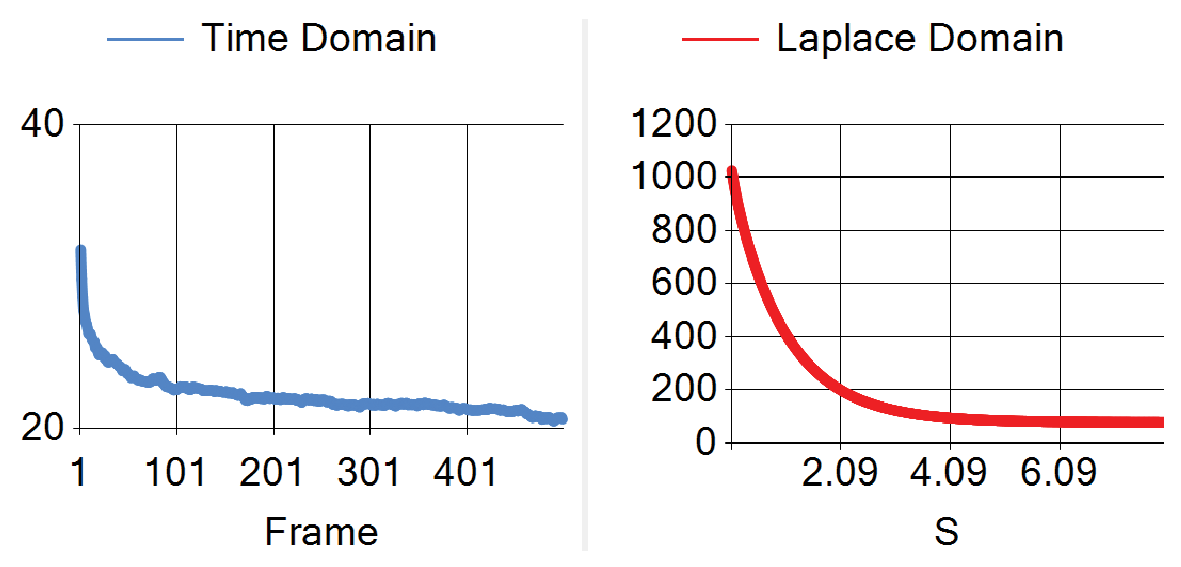
\epsfig{width=5.0in,file=Figures/ana-1.eps} &
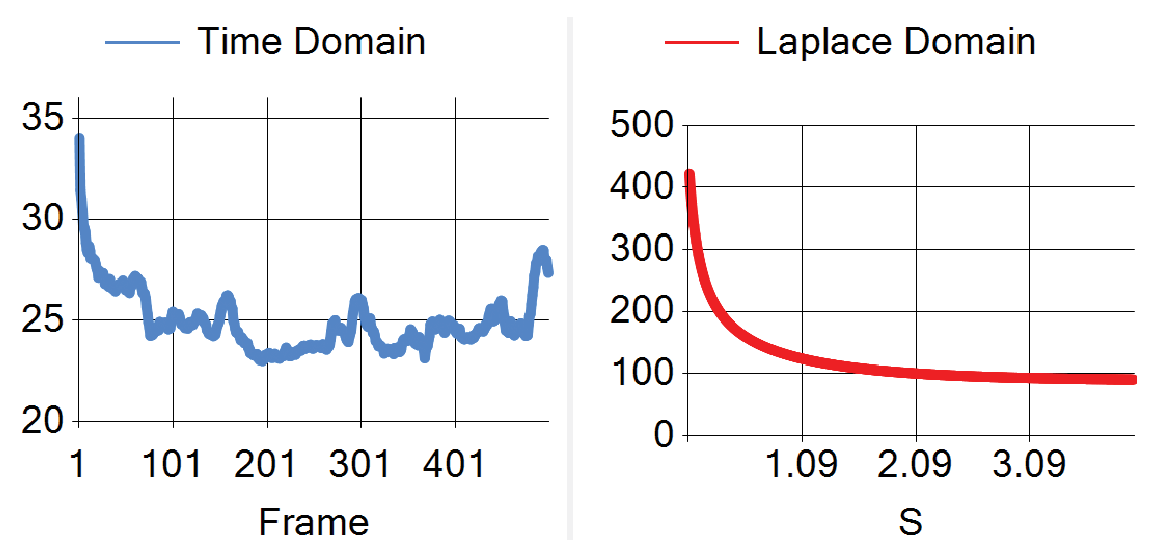
\epsfig{width=5.0in,file=Figures/ana-2.eps} \\
{\small \footnotesize{BasketballDrill (inter coding)}} & {\small \footnotesize{BasketballPass (inter coding)}}\\
\multicolumn{2}{c}{} \\[-0.5em]
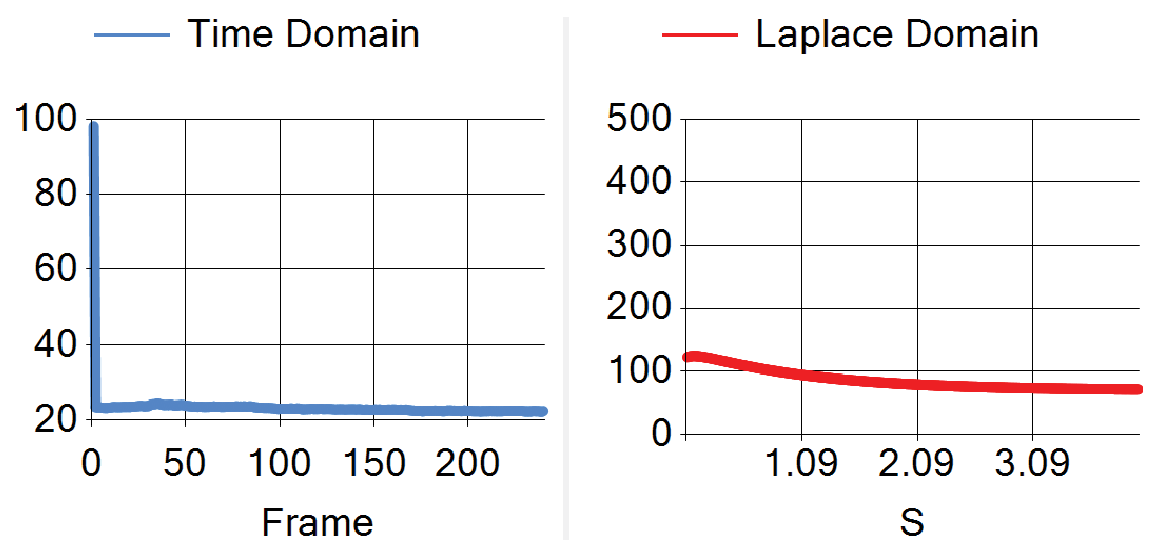
\epsfig{width=5.0in,file=Figures/ana-3-1.eps} &
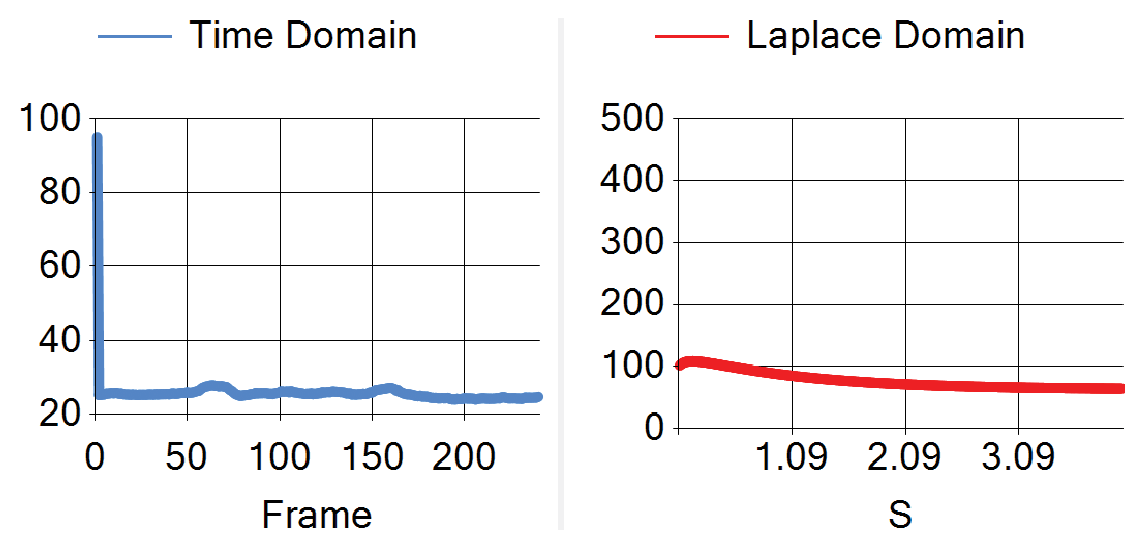
\epsfig{width=5.0in,file=Figures/ana-4-1.eps} \\
{\small \footnotesize{BlowingBubbles (intra coding)}} & {\small \footnotesize{BasketballPass (intra coding)}}\\
\end{tabular}
\label{anay}
\end{center}
\end{figure}

\begin{equation}
\label{inter-relation}
\textbf{Inter~Frame:~}A_1^\mathbb{I} \cdot e_t + A_2^\mathbb{I} \cdot \frac{de_t}{dt} = \mathrm{QP}_t,
\end{equation}
\begin{equation}
\label{intra-relation}
\textbf{Intra~Frame:~}A_0^\mathbb{I} \cdot e_t = \mathrm{QP}_t,
\end{equation}
where $A_0^\mathbb{I}$, $A_1^\mathbb{I}$ and $A_2^\mathbb{I}$ are the coefficients derived from the data analysis in Figure~\ref{anay}. Note that the exact values for $A_0^\mathbb{I}$, $A_1^\mathbb{I}$ and $A_2^\mathbb{I}$ are unnecessary, since our PQC method only requires the number of orders for the differential equations, when applying the PID controller to solve our quality control formulation of \eqref{quality-control-formulation}.

\end{block}

%----------------------------------------------------------------------------------------

\end{column} % End of column 2.1

\begin{column}{\onecolwid}\vspace{-.6in} % The second column within column 2 (column 2.2)

%----------------------------------------------------------------------------------------
%	METHODS
%----------------------------------------------------------------------------------------

\begin{block}{Our PQC Method}

The PID controller minimizes error $e_t$ alongside time $t$, via adjusting control variable $o_t$.
\begin{equation}
\label{PID-equation}
o_t=K_pe_{t-1}+K_i\int^{t-1}_0e_{\tau}d{\tau}-K_d\dfrac{de_{t-1}}{dt},
\end{equation}
However, the PID controller can perform well only when applied to a second-order system. In other words, $e_t$ and $o_t$ in \eqref{PID-equation} need to satisfy the following differential equation:

\begin{equation}
\label{pid-controller-satisfy}
M_2 \cdot \frac{d^2e_t}{dt^2} + M_1 \cdot \frac{de_t}{dt} + M_0 \cdot e_t = o_t,
\end{equation}
where $M_2$, $M_1$ and $M_0$ are coefficients. Next, we use the following way to make the modelled relationship between $e_t$ and $\mathrm{QP}_{t}$ (i.e., \eqref{inter-relation} and \eqref{intra-relation}) satisfy the above requirement of the PID controller (i.e., \eqref{pid-controller-satisfy}), such that, the PID controller can be applied to solve our quality control formulation. Specifically, by applying the differential operation on \eqref{inter-relation}, the following equation holds:
\begin{equation}
\label{weifen-tui}
A_1^\mathbb{I} \cdot \frac{d^2e_t}{dt^2} + A_0^\mathbb{I} \cdot \frac{de_t}{dt} +0 \cdot e_t= \frac{d\mathrm{QP}_t}{dt}.
\end{equation}
Thus, we can see that \eqref{weifen-tui} meets the requirement \eqref{pid-controller-satisfy} of the PID controller with $M_2=A_1^\mathbb{I}$, $M_1=A_0^\mathbb{I}$ and $M_0=0$. As a result, we have
\begin{equation}
\label{ddd}
\frac{d\mathrm{QP}_t}{dt}=o_t.
\end{equation}
Then, \eqref{ddd} can be rewritten as follows,
\begin{equation}
\mathbf{Inter~Frame:~}\mathrm{QP}_{t}=\int^t_0 o_\tau d\tau.
\end{equation}
Similarly, on the basis of \eqref{intra-relation} and \eqref{pid-controller-satisfy}, we have the following equation for the intra frames of video coding:
\begin{equation}
\mathbf{Intra~Frame:~}\mathrm{QP}_{t}=\int_0^{t}\int_0^{\tau} o_\rho d{\rho}d{\tau}.
\end{equation}
Finally, by replacing $o_t$ with \eqref{PID-equation}, the $\mathrm{QP}$ values of each frame can be estimated as follows for controlling quality of video coding.
\begin{equation}
\label{final-policy-function-inter}
\mathbf{Inter~Frame:~}\mathrm{QP}_{t}=\int_0^{t} o_\tau d{\tau},
\end{equation}
\begin{equation}
\label{final-policy-function-intra}
\mathbf{Intra~Frame:~}\mathrm{QP}_{t}=\int_0^{t}\int_0^{\tau} o_\rho d{\rho}d{\tau},
\end{equation}
Obviously, we can see that $\mathrm{QP}_t$ is only related to the control error. Thus, that our method can be seen as an encoder-free quality control method.
\end{block}
%----------------------------------------------------------------------------------------

\end{column} % End of column 2.2

\end{columns} % End of the split of column 2 - any content after this will now take up 2 columns width

%----------------------------------------------------------------------------------------
%	IMPORTANT RESULT
%----------------------------------------------------------------------------------------

%\begin{alertblock}{Important Result}
%
%Lorem ipsum dolor \textbf{sit amet}, consectetur adipiscing elit. Sed commodo molestie porta. Sed ultrices scelerisque sapien ac commodo. Donec ut volutpat elit.
%
%\end{alertblock}

%----------------------------------------------------------------------------------------

\begin{columns}[t,totalwidth=\twocolwid] % Split up the two columns wide column again

\begin{column}{\onecolwid} % The first column within column 2 (column 2.1)

%----------------------------------------------------------------------------------------
%	MATHEMATICAL SECTION
%----------------------------------------------------------------------------------------


%----------------------------------------------------------------------------------------

\end{column} % End of column 2.1

\begin{column}{\onecolwid} % The second column within column 2 (column 2.2)

%----------------------------------------------------------------------------------------
%	RESULTS
%----------------------------------------------------------------------------------------

%\begin{block}{Results}
%
%\begin{figure}
%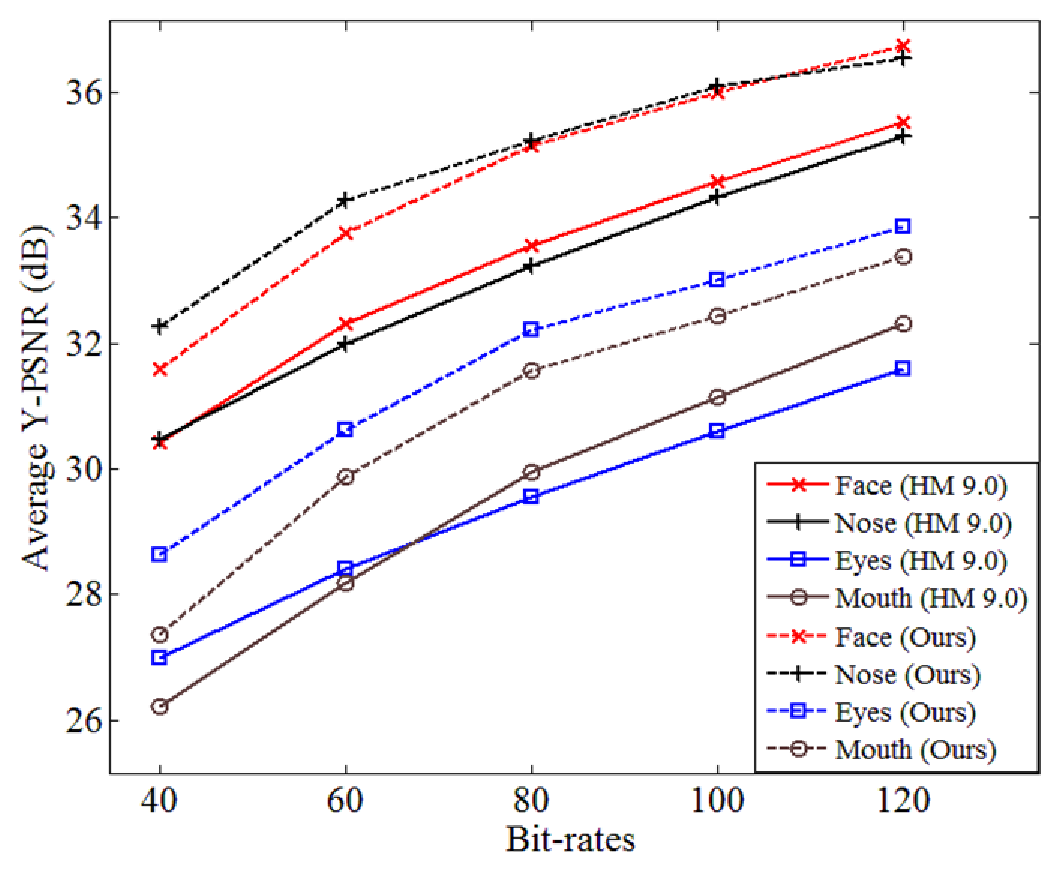
\includegraphics[width=0.8\linewidth]{foreman_features.eps}
%\caption{Figure caption}
%\end{figure}
%
%Nunc tempus venenatis facilisis. Curabitur suscipit consequat eros non porttitor. Sed a massa dolor, id ornare enim:
%
%\begin{table}
%\vspace{2ex}
%\begin{tabular}{l l l}
%\toprule
%\textbf{Treatments} & \textbf{Response 1} & \textbf{Response 2}\\
%\midrule
%Treatment 1 & 0.0003262 & 0.562 \\
%Treatment 2 & 0.0015681 & 0.910 \\
%Treatment 3 & 0.0009271 & 0.296 \\
%\bottomrule
%\end{tabular}
%\caption{Table caption}
%\end{table}
%
%\end{block}

%----------------------------------------------------------------------------------------

\end{column} % End of column 2.2

\end{columns} % End of the split of column 2

\end{column} % End of the second column

\begin{column}{\sepwid}\end{column} % Empty spacer column

\begin{column}{\onecolwid} % The third column

%----------------------------------------------------------------------------------------
%	CONCLUSION
%----------------------------------------------------------------------------------------

\begin{block}{Results}

\textbf{Quality fluctuation}:
\begin{figure}
\begin{center}
%    \caption{\footnotesize{Bit fluctuation comparison for Li \emph{et al.} \cite{bin2014lambda} and our RTE methods.}}
    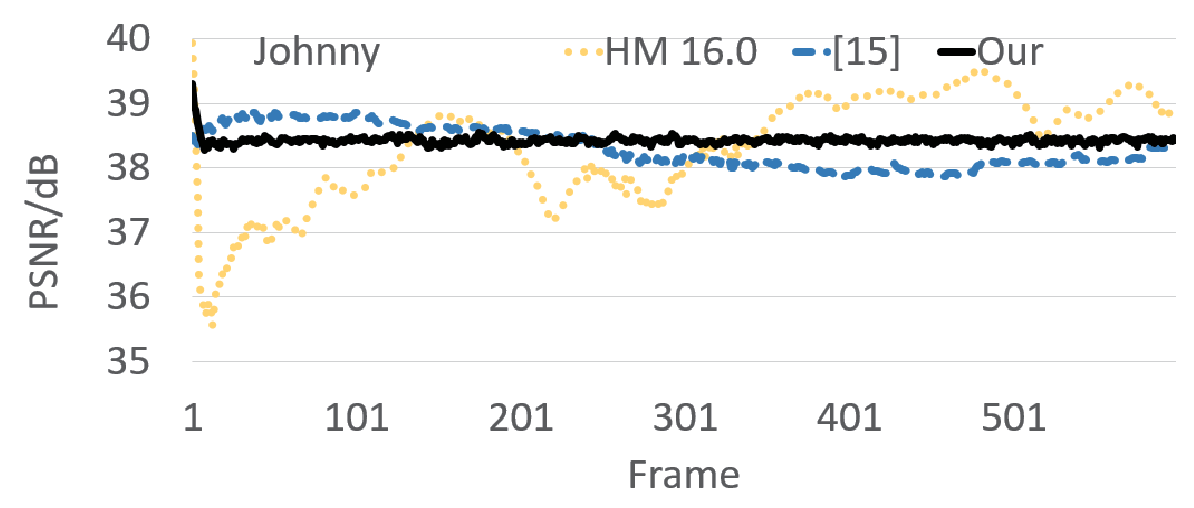
\includegraphics[width=.90\linewidth]{Figures/rs1.eps}
\label{figurebitfluctuation}
\end{center}
\end{figure}
\begin{figure}
\begin{center}
%    \caption{\footnotesize{Bit fluctuation comparison for Li \emph{et al.} \cite{bin2014lambda} and our RTE methods.}}
    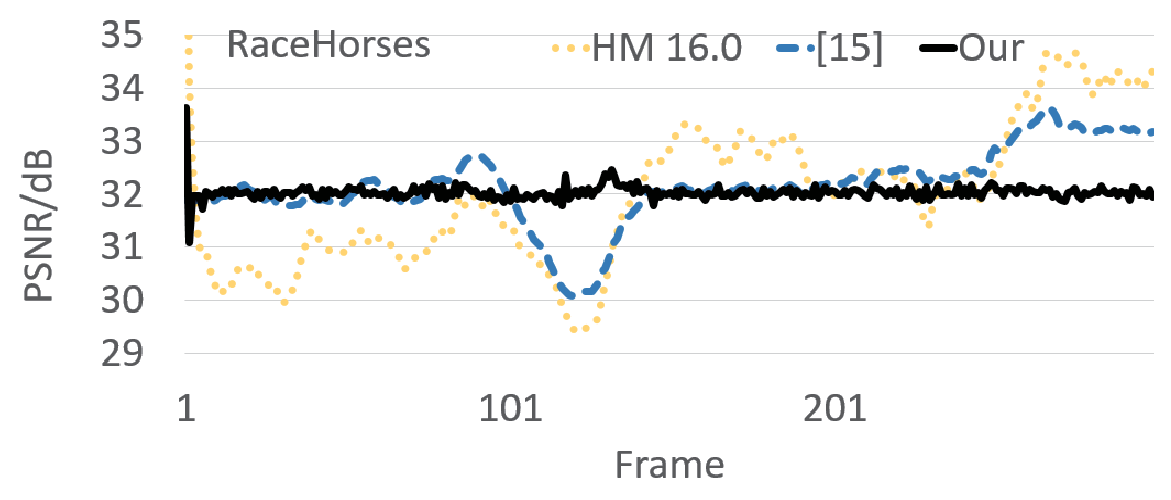
\includegraphics[width=.90\linewidth]{Figures/rs2.eps}
\label{figurebitfluctuation}
\end{center}
\end{figure}
\begin{figure}
\begin{center}
%    \caption{\footnotesize{Bit fluctuation comparison for Li \emph{et al.} \cite{bin2014lambda} and our RTE methods.}}
    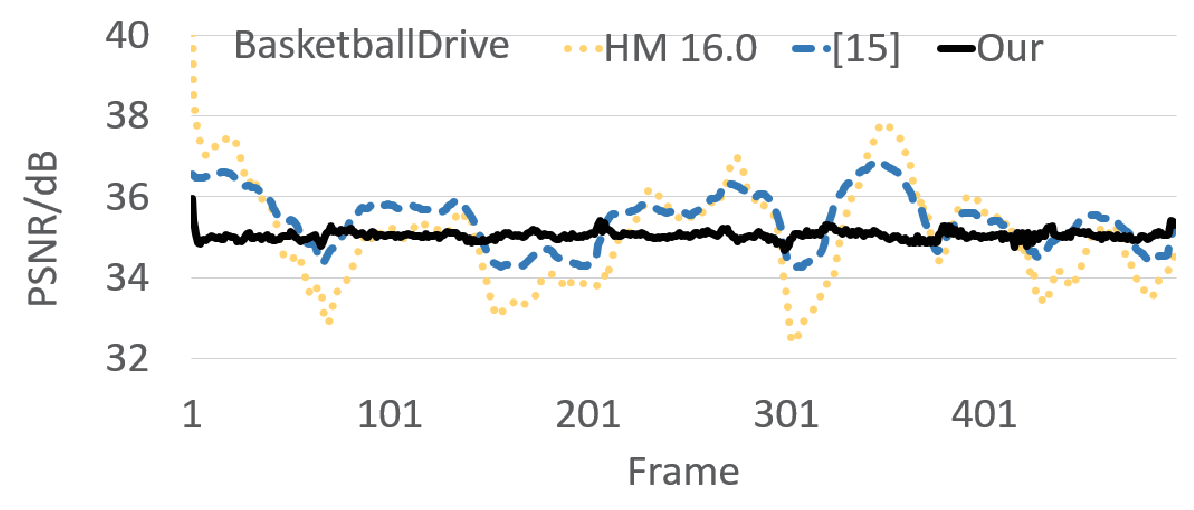
\includegraphics[width=.90\linewidth]{Figures/rs3.eps}
\label{figurebitfluctuation}
\end{center}
\end{figure}
\begin{figure}
\begin{center}
%    \caption{\footnotesize{Bit fluctuation comparison for Li \emph{et al.} \cite{bin2014lambda} and our RTE methods.}}
    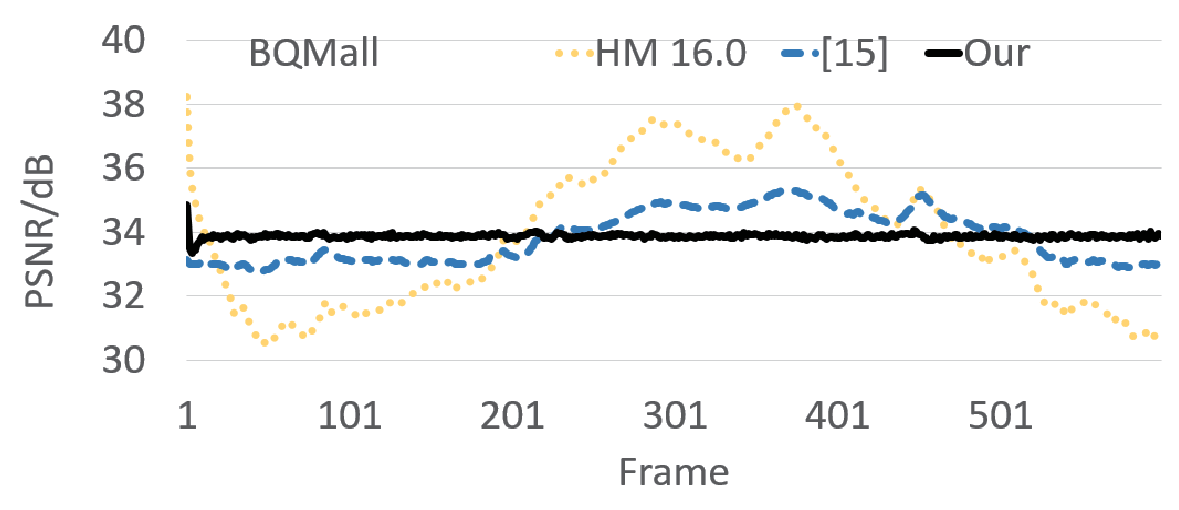
\includegraphics[width=.90\linewidth]{Figures/rs4.eps}
\label{figurebitfluctuation}
\end{center}
\end{figure}
\textbf{Bit fluctuation}:
\begin{figure}
\begin{center}
%    \caption{\footnotesize{Bit fluctuation comparison for Li \emph{et al.} \cite{bin2014lambda} and our RTE methods.}}
    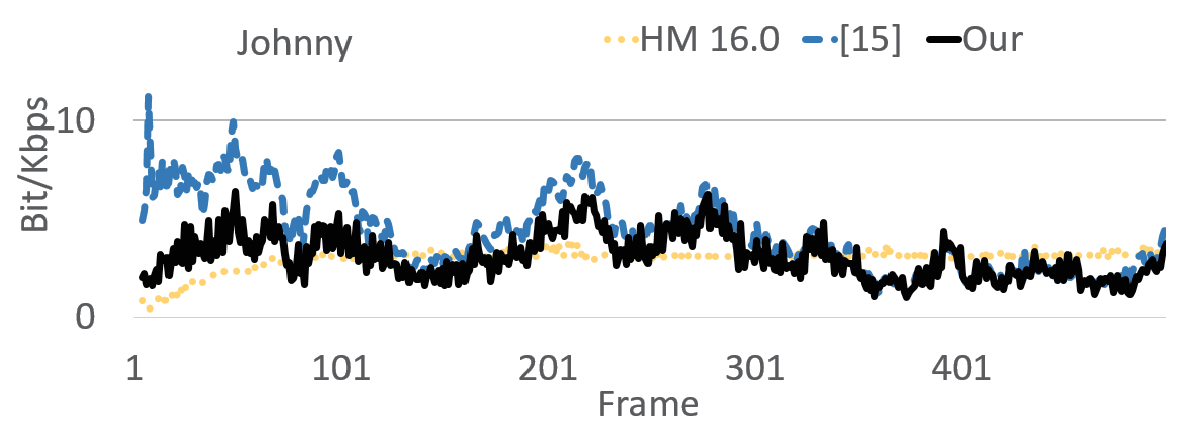
\includegraphics[width=.90\linewidth]{Figures/rsb1.eps}
\label{figurebitfluctuation}
\end{center}
\end{figure}

\end{block}

%----------------------------------------------------------------------------------------
%	ADDITIONAL INFORMATION
%----------------------------------------------------------------------------------------

%\begin{block}{Additional Information}
%
%Maecenas ultricies feugiat velit non mattis. Fusce tempus arcu id ligula varius dictum.
%\begin{itemize}
%\item Curabitur pellentesque dignissim
%\item Eu facilisis est tempus quis
%\item Duis porta consequat lorem
%\end{itemize}
%
%\end{block}

%----------------------------------------------------------------------------------------
%	REFERENCES
%----------------------------------------------------------------------------------------

%----------------------------------------------------------------------------------------
%	ACKNOWLEDGEMENTS
%----------------------------------------------------------------------------------------

\setbeamercolor{block title}{fg=red,bg=white} % Change the block title color

%----------------------------------------------------------------------------------------
%	CONTACT INFORMATION
%----------------------------------------------------------------------------------------

\setbeamercolor{block alerted title}{fg=black,bg=norange} % Change the alert block title colors
\setbeamercolor{block alerted body}{fg=black,bg=white} % Change the alert block body colors

\begin{alertblock}{Contact Information}

\begin{itemize}
\item Email: \href{YuhangSong2017@gmail.com}{YuhangSong2017@gmail.com}
\item Phone: +86 13020075391
\end{itemize}

\end{alertblock}

%----------------------------------------------------------------------------------------

\end{column} % End of the third column

\end{columns} % End of all the columns in the poster

\end{frame} % End of the enclosing frame

\end{document}
